% !TEX root = ../entropy.tex

\section{Additional results}%
\label{sec:additional_results}

\subsection{Entropy components}%
\label{sub:entropy_components}

Figure~\ref{fig:entropy_components} shows the empirical relationship with our
48-categories-based unsmoothed entropy variable and these three
components.\footnote{To highlight the main features of the relationships we
have trimmed the component values at the 95th percentile.} We can see that for
the values we observe in the dataset, entropy increases monotonically in the
number of unique spending categories with positive frequency counts, has no
clear relationship with the standard deviation of those counts, and increases
in the number of total spending transactions up to about 175 transaction,
before being increasingly determined by other elements thereafter.

\begin{figure}[ht]
    \centering 
    \caption{Correlation of entropy with its components}
    \label{fig:entropy_components}
    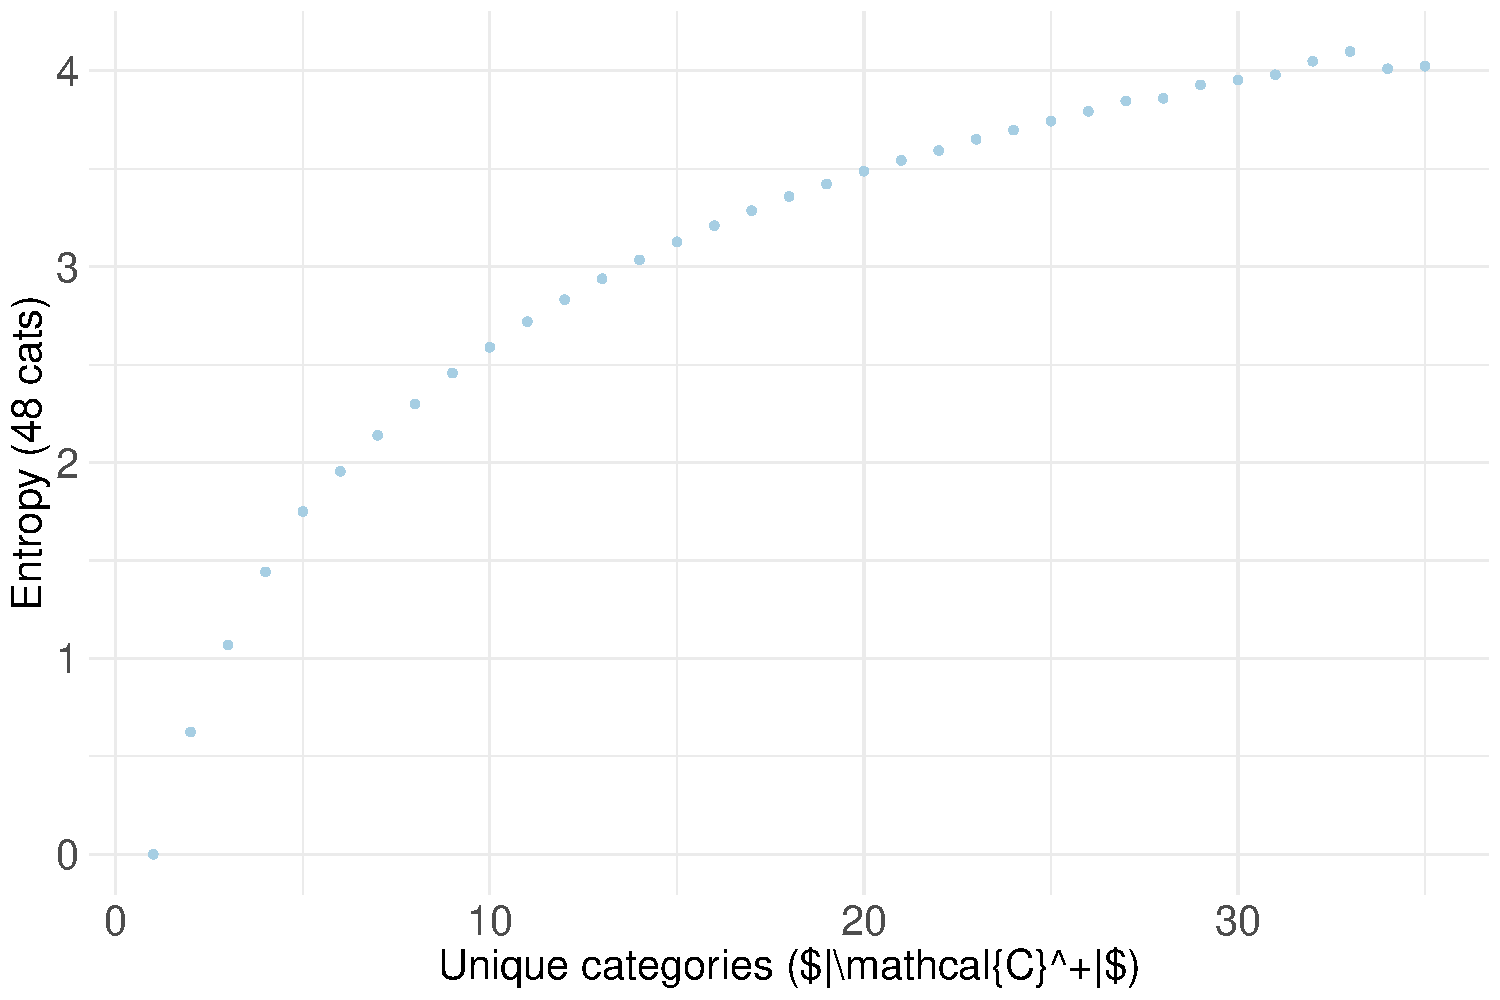
\includegraphics[width=.32\textwidth]{\figdir/scatter_entropy_nunique_tag_spend.pdf}
    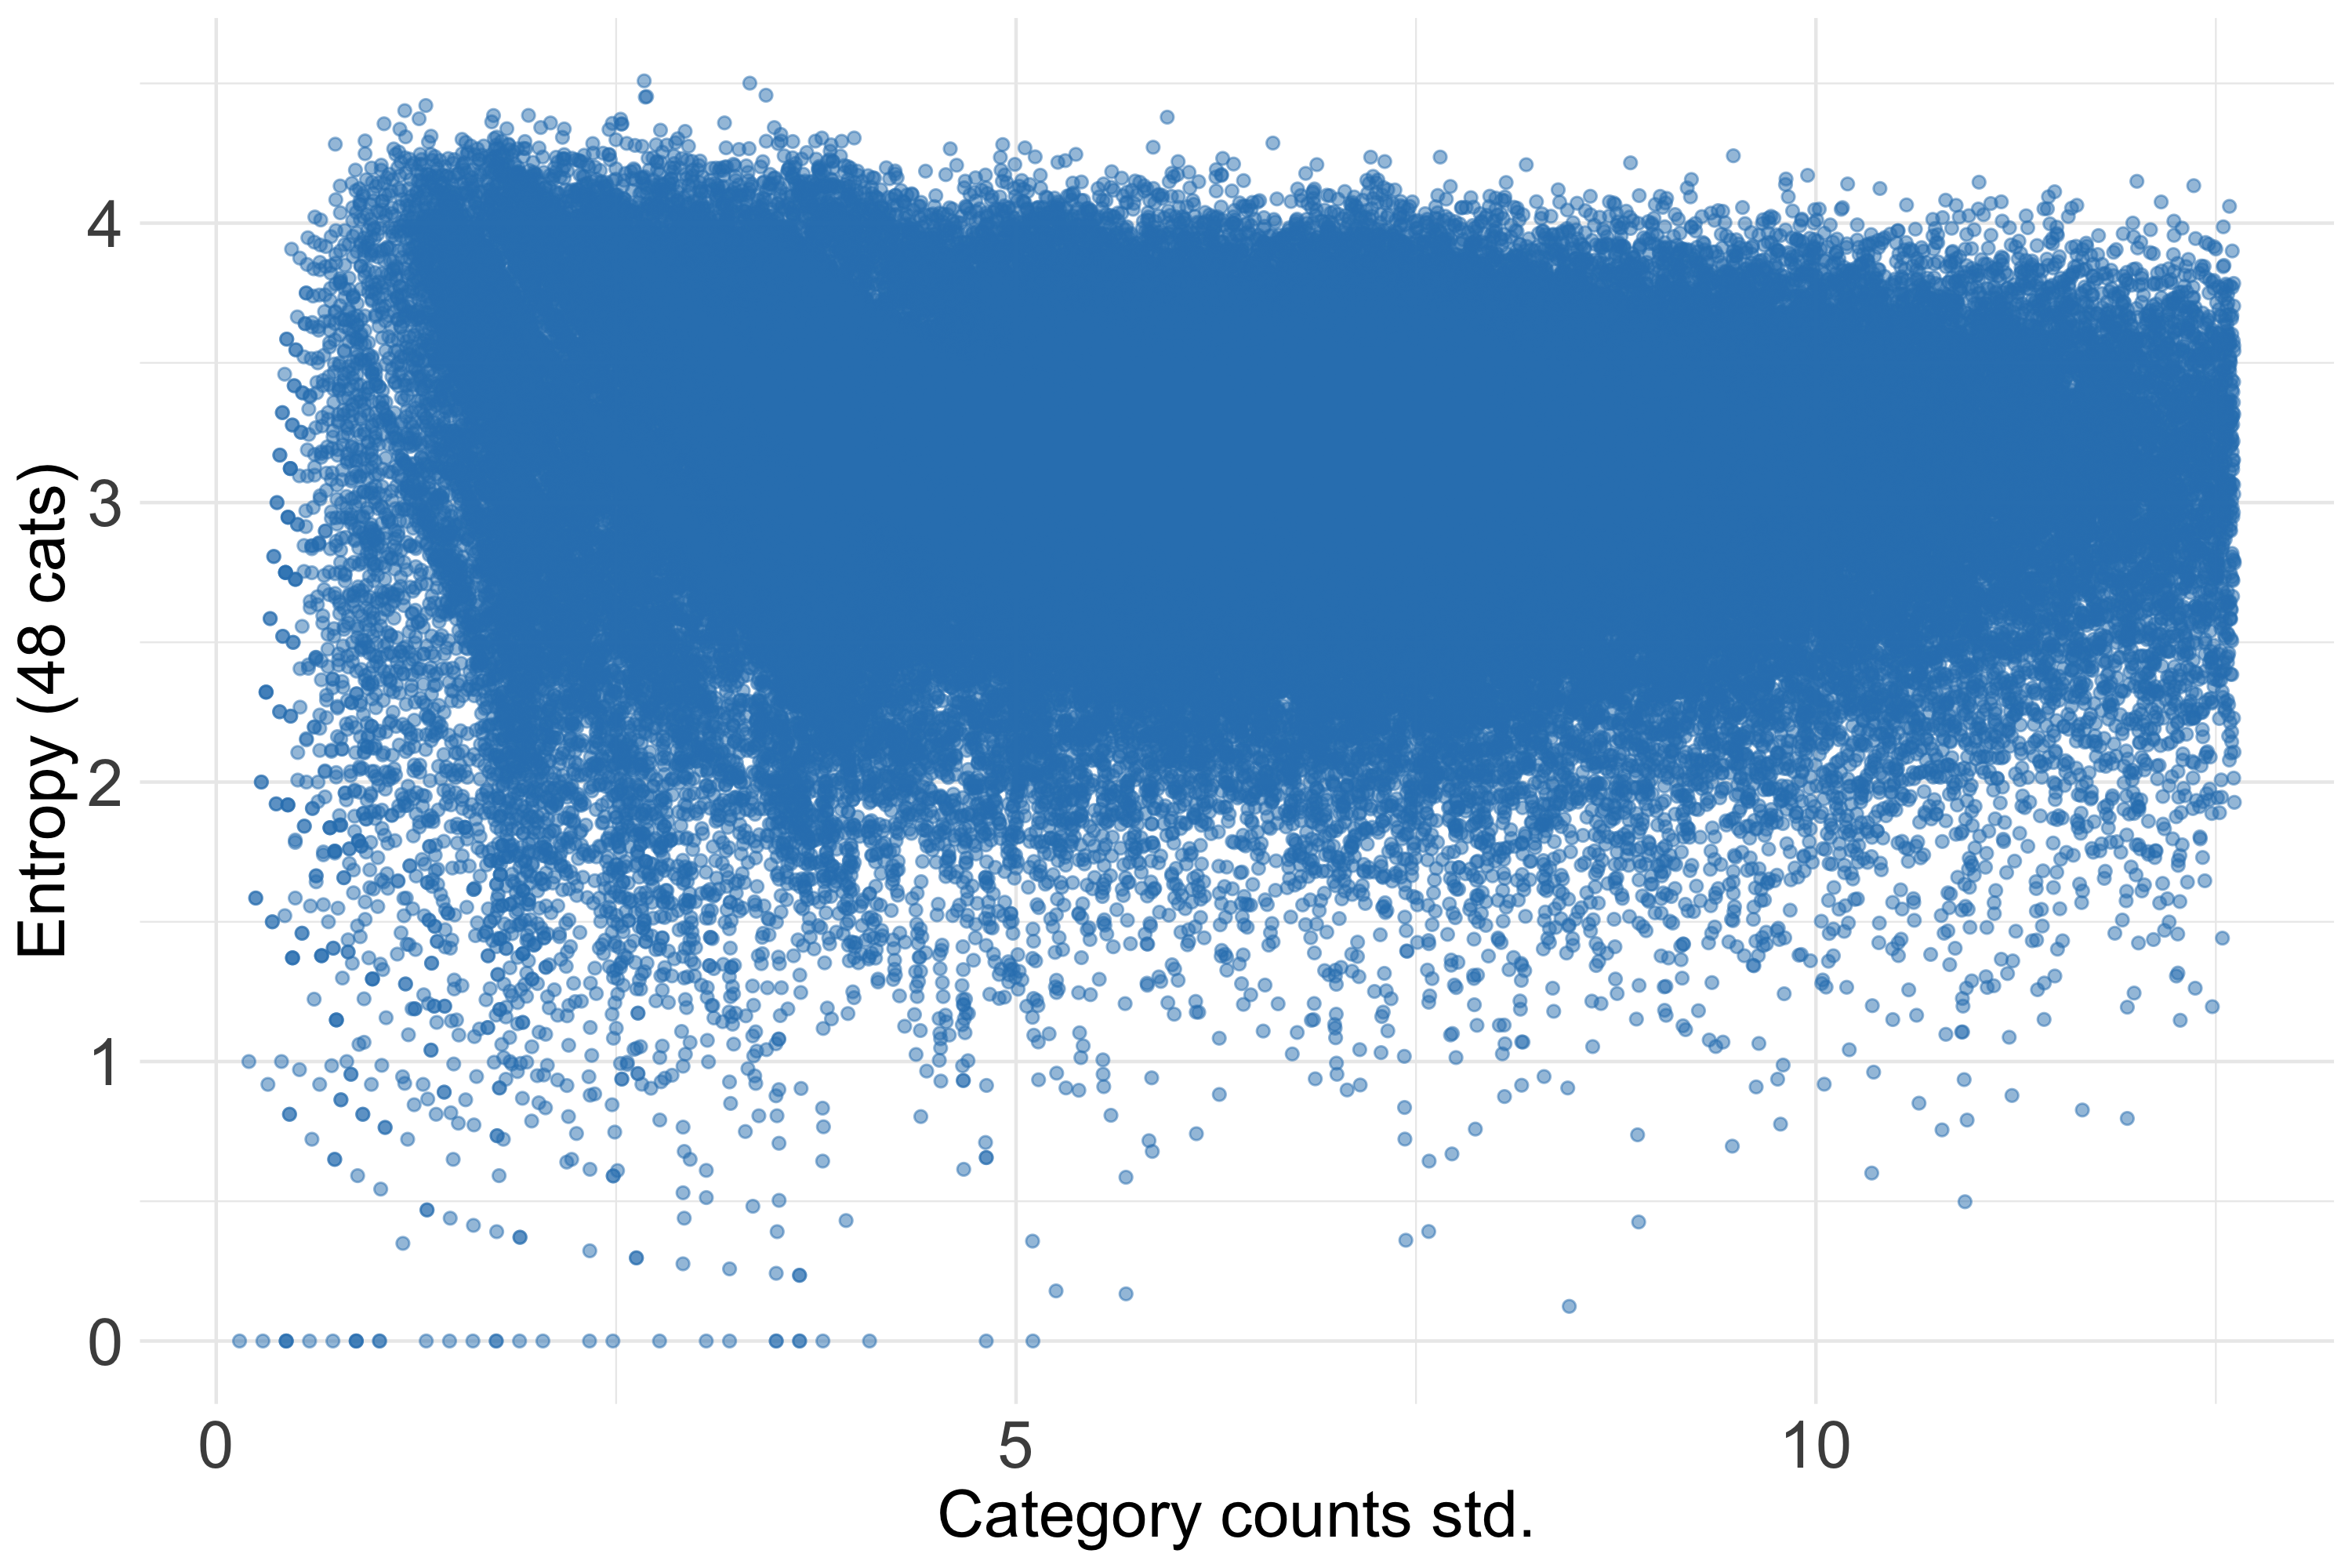
\includegraphics[width=.32\textwidth]{\figdir/scatter_entropy_std_tag_spend.pdf}
    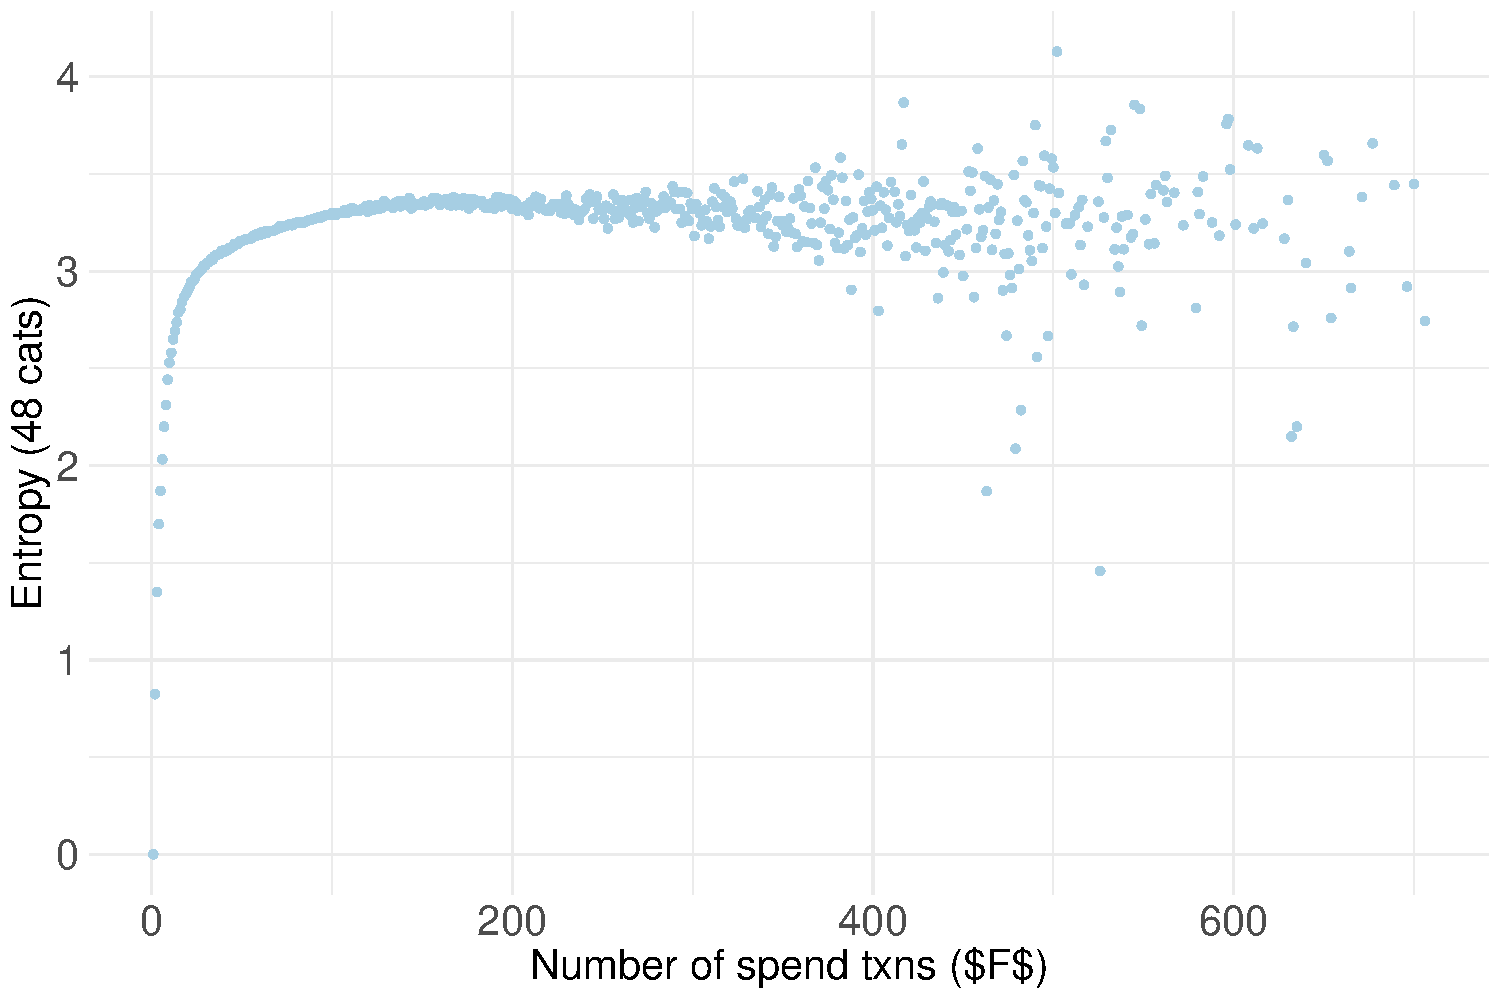
\includegraphics[width=.32\textwidth]{\figdir/scatter_entropy_txns_count_spend.pdf}
    \fignote{\textwidth}{Correlation of 48-categories-based unsmoothed entropy
    with its three main components: the number of unique spending categories
with positive frequency counts (left), the standard deviation of those
frequency counts (middle), and the number of total spend transactions (left).}
\end{figure}

\subsection{Effect of smoothing on entropy (by number of spend quintile)}%
\label{sub:effect_of_smothing_on_entropy_by_number_of_spend_quintile_}

\begin{figure}[ht]
    \centering 
    \caption{Effect of smoothing on entropy}
    \label{fig:scatter_facets_txns_count_spend_q}
    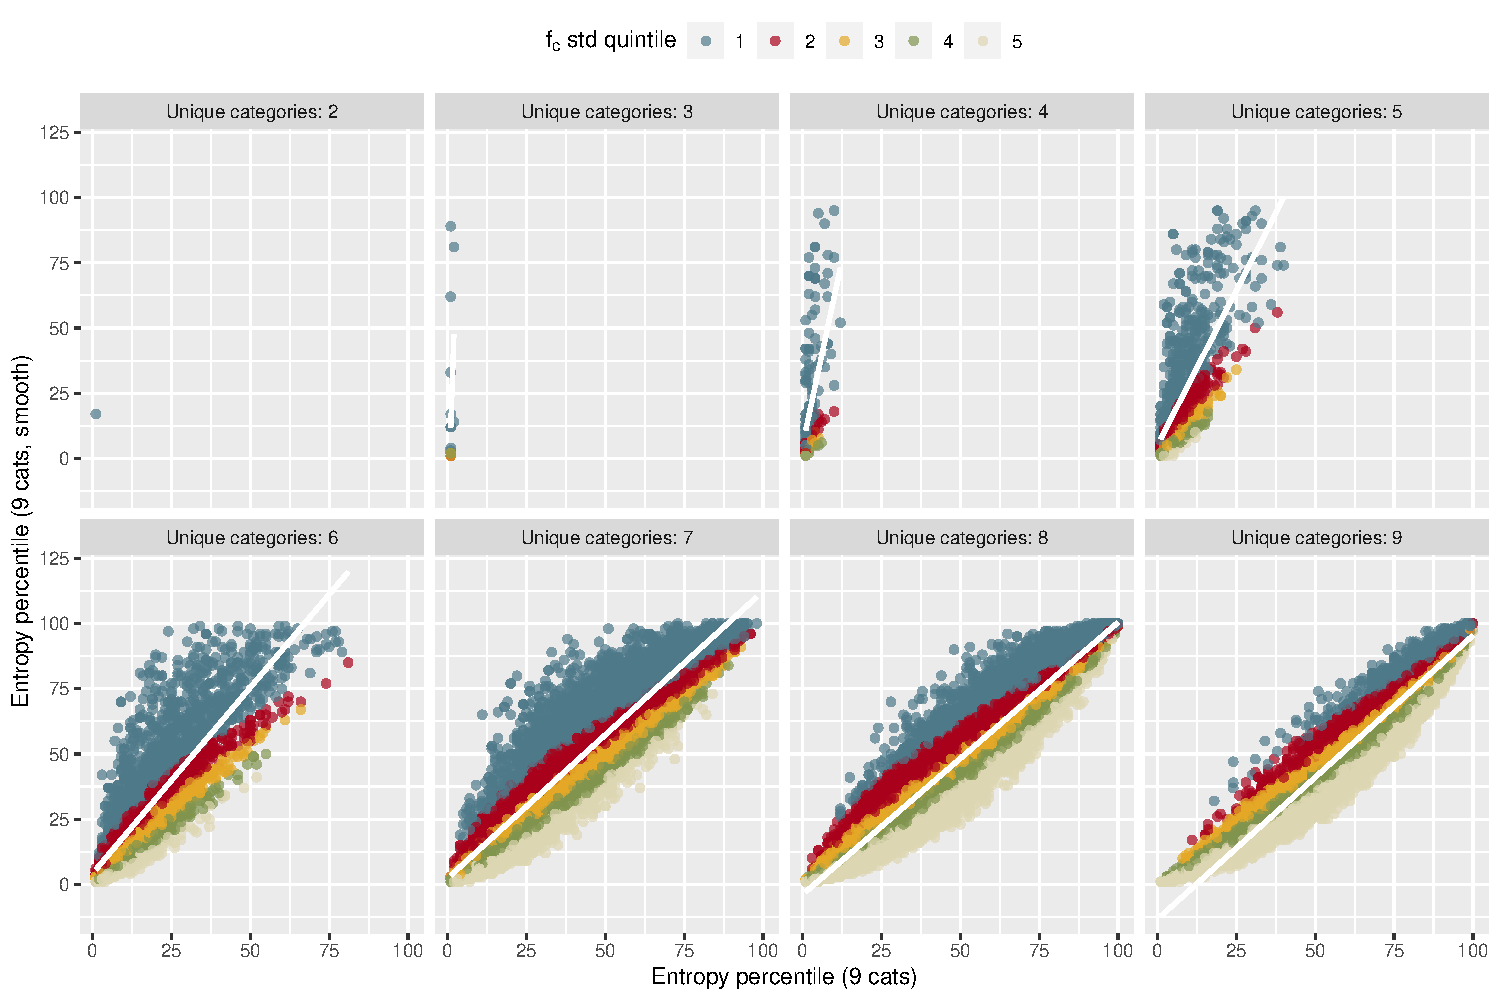
\includegraphics[width=\textwidth]{\figdir/scatter_facet_std_tag_q.pdf}
    \fignote{\textwidth}{Percentile ranks of 9-category-based unsmoothed and
    smoothed entropy separated by the number of categories with positive
frequency counts. White reference lines indicate equal percentile ranks.
Colours indicate the quintile of the total number of spending transactions.}
\end{figure}

